\chapter{Introducción y contextualización}\label{chapter:introduccion}

En la actualidad, con el auge de la inteligencia artificial (IA), surgen sin cesar nuevas herramientas destinadas a resolver problemas cuyo grado de complejidad es cada vez más elevado. En ocasiones, dicha complejidad es tal que no basta con utilizar un conjunto de algoritmos sencillos para obtener el resultado esperado, sino que se opta por emplear otras técnicas  que se basan en intentan conseguir el mejor resultado posible, respetando un cierto conjunto de reglas.

El problema principal que se plantea en este proyecto es la simulación del comportamiento humano durante un partido de pádel en un entorno virtual. Precisamente, el pádel es un deporte bastante complejo y diseñar un programa capaz de jugarlo puede llegar a complicarse bastante, teniendo en cuenta la cantidad de mecánicas de las que dispone.

Una solución a este problema es la simulación mediante agentes virtuales, los cuales son, en esencia, programas diseñados para interactuar con personas, otros agentes y/o un entorno específico que, mediante técnicas de aprendizaje automático, se les puede entrenar para atribuirles comportamientos que no son triviales de implementar.

Concretamente, en este trabajo de fin de grado (TFG) se estudian las técnicas de aprendizaje por refuerzo y por imitación, así como su aplicación en el entrenamiento de agentes virtuales en el entorno del pádel. 

\section{Contexto}

El proyecto \emph{\getTitulo} es un TFG de modalidad A (centro) que pertenece a la titulación del Grado en Ingeniería Informática, impartido por la Facultad de Informática de Barcelona (FIB) de la Universidad Politécnica de Cataluña (UPC), dentro de la mención de Computación. Este proyecto está dirigido por Carlos Andújar Gran como director y Mohammadreza Javadiha como codirector, ambos del Departamento de Ciencias de la Computación (CS).

\section{Conceptos}\label{section:conceptos}

\subsection{Aprendizaje por refuerzo}

El aprendizaje por refuerzo (RL) es un área del aprendizaje automático que utiliza agentes para tomar decisiones, premiando las acciones deseadas y penalizando las no deseadas. En general, un agente de RL es capaz de percibir e interpretar el entorno en el que se encuentra, tomar acciones basándose en su política y, como resultado, recibir recompensas y transiciones a nuevos estados. El objetivo del aprendizaje por refuerzo es, por lo tanto, aprender unas políticas óptimas que maximicen las recompensas acumuladas a largo plazo.

\begin{figure} [H]
    \centering
    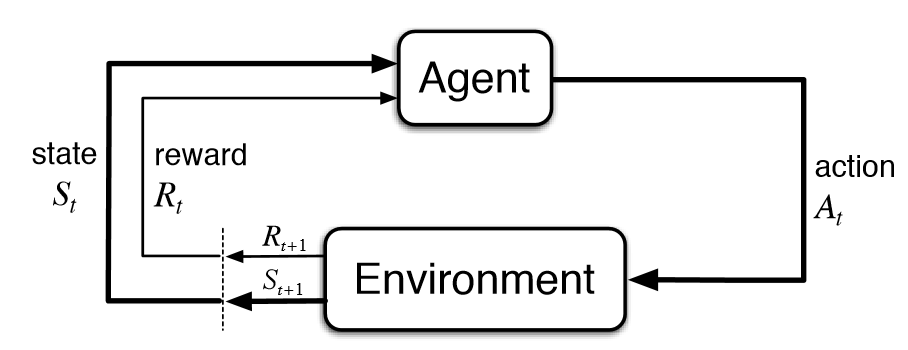
\includegraphics[width=10cm]{figures/reinforcement_learning.png}
    \caption[Flujo genérico del aprendizaje por refuerzo]{Flujo genérico del aprendizaje por refuerzo. (Fuente: \parencite{Sutton1998})}
    \label{rl_model}
\end{figure}

Formalmente, un modelo básico de RL (Figura \ref{rl_model}) consiste en: un conjunto de estados del entorno $S$; un conjunto de acciones $A$; un conjunto de recompensas $R$ y una función de transición $T$.

En cada instante $t$, el agente percibe un estado ${s}_{t}\in{S}$ y recibe un conjunto de posibles acciones para dicho estado ${A}({s}_{t})$. Luego, selecciona una acción ${a}\in{A}({s}_{t})$ y recibe del entorno un nuevo estado ${s}_{t+1}$ y una recompensa ${r}_{t+1}$, lo que significa que el agente hace una asignación de estados a probabilidades de seleccionar cada acción. Esta asignación es la política del agente y se denota como $\pi_{t}$, donde $\pi_{t}({a|s})$ es la probabilidad con la que $a_t=a$ si $s_t=s$, es decir, la probabilidad de seleccionar la acción $a$ dado el estado $s$ en el instante $t$.

La función de recompensa es la que define el objetivo en un problema de RL. El agente inteligente busca, a la larga, maximizar la recompensa recibida, por lo que debe explorar activamente su entorno y observar los efectos de sus acciones.



\subsection{Aprendizaje por imitación}

Aunque el aprendizaje por refuerzo funcione bien en muchos contextos, es necesario poder asumir que se conoce la función de recompensa, hecho que presenta algunos inconvenientes. Por una parte, determinar una función de recompensa adecuada que permita cumplir el objetivo deseado no resulta fácil. Por otra, las recompensas definidas podrían resultar ser demasiado escasas, dificultando el proceso de aprendizaje al no haber suficiente \emph{feedback} con el que se pueda guiar un agente.

Por ello, surge la necesidad de introducir el enfoque de aprendizaje por imitación (IL) en el RL, donde no se asume que la función de recompensa sea conocida de antemano, sino que se asume que dicha función de recompensa se define implícitamente mediante demostraciones o \emph{feedback} de expertos.

La formulación de un problema de IL es similar a la del RL. La principal diferencia es que, en lugar de definir explícitamente una función de recompensa, se asume que se proporciona un conjunto de demostraciones realizadas por un experto, donde cada demostración  $\xi$ consiste en una secuencia de pares de estados y acciones $\xi=\{(s_0, a_0), (s_1, a_1), ...\}$.

En un problema de IL, en contraste a un problema de RL, el agente inteligente debe buscar la política $\pi$ que más se asemeja a la política de un experto $\pi^*$. La política del experto no se puede observar directamente, sino que se trata de aproximar a través de las demostraciones.

\section{Identificación del problema}

En este trabajo se desarrolla una aplicación que permite simular partidos de pádel en un entorno virtual, por lo que el problema se ha dividido en dos grandes bloques. Por una parte está el diseño y desarrollo de un entorno virtual de pádel y, por otra, la simulación de agentes capaces de jugar a pádel.

\subsection{Diseño y desarrollo de un entorno virtual de pádel}

El entorno virtual de pádel es una pieza clave en este proyecto, ya que determina lo fieles que serán las simulaciones respecto a la realidad. Por esta razón, el diseño de este entorno se debe hacer meticulosamente, respetando lo máximo posible el entorno físico en el que se basa, para poder transmitir cierta sensación de realismo.

El diseño no implica únicamente la estructura de una pista de pádel, sino que también se ha de tener en cuenta todas las leyes físicas que hay detrás, ya sea de los impactos, los rebotes, las trayectorias de la pelota o el movimiento de los jugadores.

El proceso de desarrollo debe llevarse a cabo teniendo en cuenta las normas del pádel, lo cual implica la implementación de toda una serie de estados que tienen lugar a lo largo de un partido, como por ejemplo el inicio y final de un punto, las posiciones de saque o las condiciones para ganar un punto. Además de los estados, también se deben tener presentes todos los parámetros requeridos de cara a la integración de los agentes, ya que estos serán necesarios para su entrenamiento.

\subsection{Simulación de agentes capaces de jugar a pádel}

Una vez finalizado todo el proceso de diseño y desarrollo del entorno virtual, se integran los agentes para poder simular partidos de pádel. Estos agentes deben seguir un conjunto de reglas a la hora de decidir qué hacer durante el trascurso de un partido: hacia dónde moverse, qué tipo de golpeo hacer y hacia qué dirección dirigir la pelota.

Atribuir un comportamiento así únicamente mediante programación imperativa, habiendo una infinidad de posibles estados, puede llegar a ser una tarea muy laboriosa, debido al grado de complejidad presente en este deporte. Es por este motivo que se explora el uso de distintas técnicas de aprendizaje por refuerzo y por imitación para el entrenamiento de agentes virtuales, para tratar de simplificar la resolución de este problema.

\newpage

\section{Agentes implicados}

El producto desarrollado va dirigido a una gran variedad de usuarios dependiendo del uso que se le quiera dar, por ejemplo:

\begin{itemize}
    \item[-] A jugadores, entrenadores o analistas del pádel, ya que puede ser útil a la hora de estudiar los movimientos de los agentes, partiendo del análisis del entorno  junto a la decisión que acaba tomando un agente, permitiendo un estudio de jugadas que quizás no se han llegado a contemplar anteriormente. En especial, el modelo entrenado con aprendizaje por imitación, que busca simular el comportamiento de jugadores profesionales, puede servir para analizar la probabilidad de que un jugador tome ciertas decisiones dada una situación en concreto.
    \item[-] A desarrolladores de videojuegos y videojugadores, pues es un producto que se podría integrar perfectamente en un videojuego relacionado con el pádel. Sería interesante especialmente en  un videojuego de realidad virtual donde, aprovechándose de la captura de movimientos, el videojugador pueda competir contra agentes que han aprendido a seguir unas políticas óptimas, o bien han aprendido las políticas que siguen ciertos jugadores profesionales del pádel. De esta manera, el videojugador podría entrenar sus habilidades en el pádel mediante simulaciones de partidos bastante fieles a la realidad.
    \item[-] A investigadores interesados en el aprendizaje por refuerzo y/o aprendizaje por imitación, dado que puede servir como un punto de partida para una futura investigación con unos fines parecidos a los de este proyecto.
\end{itemize}

En cuanto a los beneficiarios de los resultados del producto, se puede apreciar que todos los usuarios mencionados se pueden favorecer de una manera u otra. A nivel personal también ha sido beneficioso, ya que todo el proceso de diseño, desarrollo y gestión ha servido para profundizar los conocimientos en este campo de estudio.

Además de los usuarios finales, otros agentes implicados es el equipo docente que hay detrás de este proyecto, el cual se ha encargado de orientar y supervisar las tareas realizadas durante el trascurso de este TFG.

\begin{figure}[H]
    \centering
    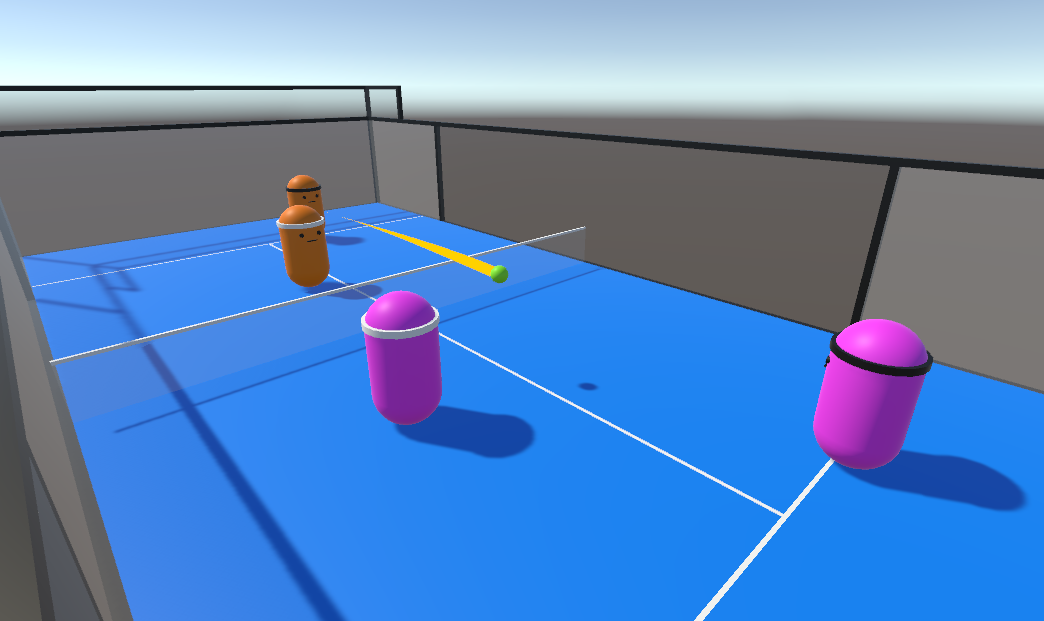
\includegraphics[width=13cm]{figures/padel-in-game.png}
    \caption[Entorno virtual de pádel]{Entorno virtual de pádel. (Elaboración propia)}
\end{figure}